\documentclass{fiwthesis}
%\documentclass[en]{fiwthesis}   % Default language is german but can be switched to english

% ========
%  Pakete
% ========

\usepackage{textgreek}           % griechische Buchstaben außerhalb des Math-Mode
\usepackage{amsmath}             % zentrierte Formeln
\usepackage{amssymb}             % erweiterter Formelsatz mathem. Symbole

\usepackage{boldline}            % breitere Linien in Tabellen
\usepackage{booktabs}            % typographisch richtige Tabellen setzen
\usepackage{tabularx}            % Erweiterte Tabellendarstellung
\usepackage{multirow}            % Spalte über mehrere Zeilen oder Spalten ausdehnen
\usepackage{xltabular}           % Zeilenumbrüche in tabularx erlauben

\usepackage{graphicx}            % ermöglicht das Einbinden von Grafiken
\usepackage{subcaption}          % mehrere Bilder in einem Bild
\usepackage{pgfplots}            % Grafiken erzeugen
\usepackage{smartdiagram}        % schnelle und einfache Grafiken
\usepackage{pdfpages}            % Einbinden von PDFs
\usetikzlibrary{positioning}     % bessere Ortsbezeichnung
\usetikzlibrary{shapes}          % typische Formen wie Rechtecke, Ellipsen usw. einfach zeichnen
\usetikzlibrary{intersections}   % Schnittpunkt von Geraden adressieren
\usetikzlibrary{angles, quotes}  % einfacheres Zeichnen von Winkeln
\usetikzlibrary{                 % Symbole für Schaltpläne
  circuits.logic.US,
  circuits.logic.IEC,
  circuits.logic.CDH,
  circuits.ee.IEC
}

\usepackage{lipsum}

% ===========
%  Metadaten
% ===========

\thesis{Master-Thesis}
\title{Identifikation und Vergleich von Autorenangaben zu Software zwischen verschiedenen Datenquellen}
\author{Kevin Jahrens}
\date{\today}
\matrnr{480592}
\bdate{05.08.1999}
\bcity{Bad Oldesloe}
\supervisor{Prof.~Dr.~-Ing.~Frank Krüger} 
\secsupervisor{M.A.~Stephan Druskat}
\keywords{Data, Science, Software, Author, Comparison, Identification}

% Metadaten in die PDF-Datei schreiben
\makepdfmetadata

% ==========
%  Präambel
% ==========

% PGF Kompatibilitätseinstellung
\pgfplotsset{width=0.95\textwidth,compat=newest}

% % Bibliographie einbinden
\bibliography{quellen}

% Glossar einbinden
\newglossaryentry{nosql}{%
  name = {NoSQL},
  description = {Kurzform für ,,Not Only SQL``; Überbegriff für Datenbanken, die das Konzept relationaler Datenbanken erweitern}
}

\newdualentry{dos}% label
{DoS}% short form
{Denial of Service}% long form
{Ein Denial of Service (im Deutschen: Dienstverweigerung) ist ein Angriffe auf Computer- oder Netzwerksysteme, wobei das Zielsystem durch Überlastung oder durch andere Mittel außer Betrieb gesetzt wird}% description

% Abkürzungen einbinden
%\gls{}         normal zu nutzen (erstes Mal: 'lange Form (kurze Form)'), danach nur 'kurze Form'
%\glspl{}       wie \gls{} nur als Plural
%\acrfull{qrc}  gibt volle Form ('lange Form (kurze Form)') egal wo
%\acrlong{qrc}  gibt lange Form ('lange Form') egal wo
%
%\newacronym{tag}{short}{long}
\newacronym{cff}{CFF}{Citation File Format}
\newacronym{pep}{PEP}{Python Enhancement Proposal}
\newacronym{pypi}{PyPI}{Python Package Index}
\newacronym{cran}{CRAN}{Comprehensive R Archive Network}
\newacronym{ner}{NER}{Named entity recognition}
\newacronym{ned}{NED}{Named entity disambiguation}
\newacronym{oss}{OSS}{Open-Source-Software}
\newacronym{doi}{DOI}{Digitaler Objektbezeichner}


% Symbole einbinden
\newglossaryentry{symb:phi}{
  name=$\phi$,
  description={Ein beliebiger Winkel},
  sort=symbolphi, type=symbolslist
}

\newglossaryentry{symb:e}{
  name=$e$,
  description={Die Eulersche Zahl},
  sort=symbole, type=symbolslist
}


% Glossar- und Abkürzungsverzeichniserstellung
\makeglossaries{}

% Index erzeugen
\makeindex[
  intoc=true,
  title=Index,
  columns=2]{}
\indexsetup{headers={\indexname}{\indexname}}

% ===============
%  Eigene Makros
% ===============

\newcommand*{\code}[1]{\texttt{#1}}

% ===============
%  Beginn Thesis
% ===============

\begin{document}

% ============
%  "Vorspann"
% ============

% Titelseite
\maketitle

% Aufgabenstellung
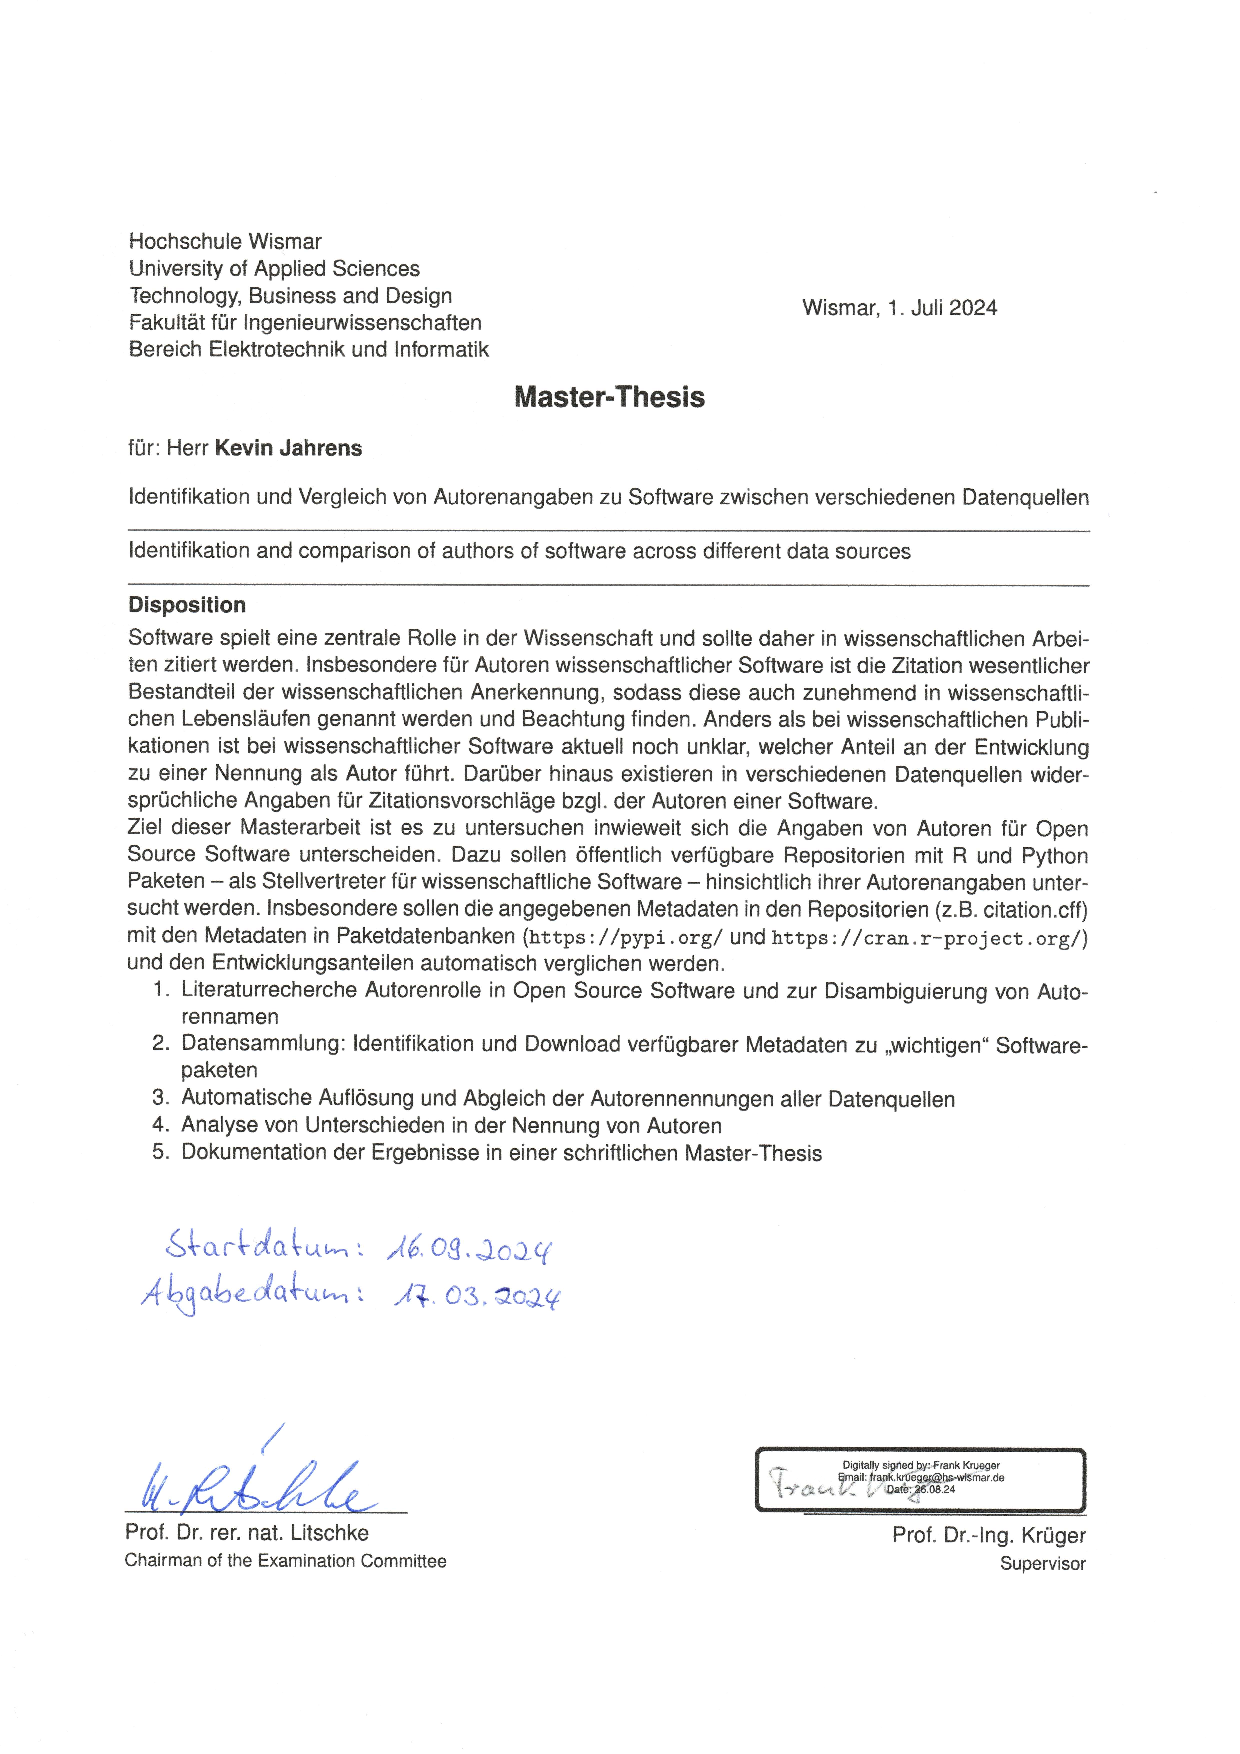
\includepdf[pages=-]{anlagen/aufgabenstellung_print.pdf}

% Abstract
\makeabstract{
  Maximal eine halbe Seite.
}

% Inhaltsverzeichnis (Schalter `compact' sorgt für einfachen Zeilenabstand)
\maketoc[compact]

% ==========
%  Textteil
% ==========

% Einleitung
\chapter{Einleitung}
\label{chap:einleitung}
\section{Motivation}
\label{sec:motivation}
\section{Vorgehen}
\label{sec:vorgehen}
% TODO erklären was wird vorhaben (Autoren aus unterschiedlichen quellen extrahieren zuordnen und checken wie gut das funktioniert und wie gut Autoren von Software gepflegt werden)
\section{Gliederung}
\label{sec:gliederung}


% weitere Kapitel hier jeweils einzeln einbinden
\chapter{Zusätzliche Abbildungen}
\label{chap:zusaetzliche_abbildungen}

\begin{figure}[H]
    \begin{subfigure}{.5\textwidth}
        \centering
        \includesvg[width=.95\linewidth,inkscapelatex=false]{bilder/common_authors/1_pypi.svg}
        \caption{\gls{pypi} nach Commits}
        \label{fig:common_authors_pypi}
    \end{subfigure}%
    \begin{subfigure}{.5\textwidth}
        \centering
        \includesvg[width=.95\linewidth,inkscapelatex=false]{bilder/common_authors_by_files/1_pypi_by_files.svg}
        \caption{\gls{pypi} nach geänderten Zeilen}
        \label{fig:common_authors_by_files_pypi}
    \end{subfigure}
    \begin{subfigure}{.5\textwidth}
        \centering
        \includesvg[width=.95\linewidth,inkscapelatex=false]{bilder/common_authors/1_cran.svg}
        \caption{\gls{cran} nach Commits}
        \label{fig:common_authors_cran}
    \end{subfigure}%
    \begin{subfigure}{.5\textwidth}
        \centering
        \includesvg[width=.95\linewidth,inkscapelatex=false]{bilder/common_authors_by_files/1_cran_by_files.svg}
        \caption{\gls{cran} nach geänderten Zeilen}
        \label{fig:common_authors_by_files_cran}
    \end{subfigure}
    \begin{subfigure}{.5\textwidth}
        \centering
        \includesvg[width=.95\linewidth,inkscapelatex=false]{bilder/common_authors/1_cff.svg}
        \caption{\gls{cff} nach Commits}
        \label{fig:common_authors_cff}
    \end{subfigure}%
    \begin{subfigure}{.5\textwidth}
        \centering
        \includesvg[width=.95\linewidth,inkscapelatex=false]{bilder/common_authors_by_files/1_cff_by_files.svg}
        \caption{\gls{cff} nach geänderten Zeilen}
        \label{fig:common_authors_by_files_cff}
    \end{subfigure}
    \caption{Anteil der Top Git Autoren in der Zitation}
    \label{fig:common_authors_anhang}
\end{figure}


% Schluss
\chapter{Fazit und Ausblick}
\label{cap:fazit_ausblick}
\section{Fazit}
\label{sec:fazit}
\section{Ausblick}
\label{sec:ausblick}


% =========
%  Anlagen
% =========

\begin{appendices}

  \chapter{Zusätzliche Abbildungen}
\label{chap:zusaetzliche_abbildungen}

\begin{figure}[H]
    \begin{subfigure}{.5\textwidth}
        \centering
        \includesvg[width=.95\linewidth,inkscapelatex=false]{bilder/common_authors/1_pypi.svg}
        \caption{\gls{pypi} nach Commits}
        \label{fig:common_authors_pypi}
    \end{subfigure}%
    \begin{subfigure}{.5\textwidth}
        \centering
        \includesvg[width=.95\linewidth,inkscapelatex=false]{bilder/common_authors_by_files/1_pypi_by_files.svg}
        \caption{\gls{pypi} nach geänderten Zeilen}
        \label{fig:common_authors_by_files_pypi}
    \end{subfigure}
    \begin{subfigure}{.5\textwidth}
        \centering
        \includesvg[width=.95\linewidth,inkscapelatex=false]{bilder/common_authors/1_cran.svg}
        \caption{\gls{cran} nach Commits}
        \label{fig:common_authors_cran}
    \end{subfigure}%
    \begin{subfigure}{.5\textwidth}
        \centering
        \includesvg[width=.95\linewidth,inkscapelatex=false]{bilder/common_authors_by_files/1_cran_by_files.svg}
        \caption{\gls{cran} nach geänderten Zeilen}
        \label{fig:common_authors_by_files_cran}
    \end{subfigure}
    \begin{subfigure}{.5\textwidth}
        \centering
        \includesvg[width=.95\linewidth,inkscapelatex=false]{bilder/common_authors/1_cff.svg}
        \caption{\gls{cff} nach Commits}
        \label{fig:common_authors_cff}
    \end{subfigure}%
    \begin{subfigure}{.5\textwidth}
        \centering
        \includesvg[width=.95\linewidth,inkscapelatex=false]{bilder/common_authors_by_files/1_cff_by_files.svg}
        \caption{\gls{cff} nach geänderten Zeilen}
        \label{fig:common_authors_by_files_cff}
    \end{subfigure}
    \caption{Anteil der Top Git Autoren in der Zitation}
    \label{fig:common_authors_anhang}
\end{figure}


\end{appendices}

% ===============
%  Verzeichnisse
% ===============

% Verzeichnisse mit einzeiligem Zeilenabstand
\singlespacing

% Literaturverzeichnis
\listofreferences

% Abbildungsverzeichnis einfügen
\listoffigures

% Tabellenverzeichnis einfügen
\listoftables

% Algorithmenverzeichnis einfügen
\listofalgorithms

% % Quelltextverzeichnis einfügen
\listoflistings

% Abkürzungsverzeichnis
\listofacronyms

% Symbolverzeichnis
\listofsymbols

% falls ein anderer Glossar-Stil genutzt wird und die zweite Spalte zu schmal ist:
% \setlength{\glsdescwidth}{0.8\linewidth}

% Glossar einfügen
\printglossary

% Index einfügen
\printindex

% wieder auf 1½-fachen Zeilenabstand umschalten
\normalspacing

% =========================================
%  Selbstständigkeitserklärung, CD, Thesen
% =========================================

% Inhalt der CD; nur für gedruckte Version wichtig
\makecd{\small

\begin{minipage}[t]{0.97\linewidth}
  \dirtree{%
    .1 /\DTcomment{Wurzelverzeichnis}.
    .2 OrdnerA\DTcomment{Ein Ordner auf dem Datenträger}.
    .3 OrdnerB\DTcomment{Ein Unterordner auf dem Datenträger}.
    .3 datei.xyz\DTcomment{Eine Datei}.
    .2 thesis.pdf\DTcomment{PDF-Datei dieser Bachelor-Thesis}.
  }
\end{minipage}

\vspace{2em}

Im Unterverzeichnis \code{tools} des Projekts findet sich das Perl-Skript \code{dirtree.pl}, mit welchem Inhalte für das dirtree-Environment (siehe oberhalb) semiautomatisch erstellt werden können.

Die Nutzung aus der Kommandozeile ist wie folgt:\\
\code{perl dirtree.pl /path/to/top/of/dirtree}

Quelle des Skripts:\\
\url{https://texblog.org/2012/08/07/semi-automatic-directory-tree-in-latex/}
\normalsize}

% Selbstständigkeitserklärung
\makedoiw

\end{document}

% =============
%  Ende Thesis
% =============
